% UE Localization Model Architecture Diagram
% Standalone TikZ figure - compile with: pdflatex architecture_diagram.tex
% Or include in main paper with % UE Localization Model Architecture Diagram
% Standalone TikZ figure - compile with: pdflatex architecture_diagram.tex
% Or include in main paper with % UE Localization Model Architecture Diagram
% Standalone TikZ figure - compile with: pdflatex architecture_diagram.tex
% Or include in main paper with % UE Localization Model Architecture Diagram
% Standalone TikZ figure - compile with: pdflatex architecture_diagram.tex
% Or include in main paper with \input{figures/architecture_diagram.tex}

\documentclass[border=5pt]{standalone}
\usepackage{tikz}
\usetikzlibrary{positioning, arrows.meta, shapes.geometric, fit, calc, backgrounds, decorations.pathreplacing, patterns}
\usepackage{amsmath}
\usepackage{xcolor}

% Define colors matching the implementation
\definecolor{inputblue}{RGB}{66, 133, 244}
\definecolor{embedgreen}{RGB}{52, 168, 83}
\definecolor{transformerorange}{RGB}{251, 188, 5}
\definecolor{fusionpurple}{RGB}{142, 68, 173}
\definecolor{coarsered}{RGB}{234, 67, 53}
\definecolor{fineyellow}{RGB}{255, 193, 7}
\definecolor{outputteal}{RGB}{0, 150, 136}
\definecolor{mapblue}{RGB}{33, 150, 243}
\definecolor{cfrcyan}{RGB}{0, 188, 212}
\definecolor{lightgray}{RGB}{245, 245, 245}
\definecolor{darkgray}{RGB}{66, 66, 66}

\begin{document}
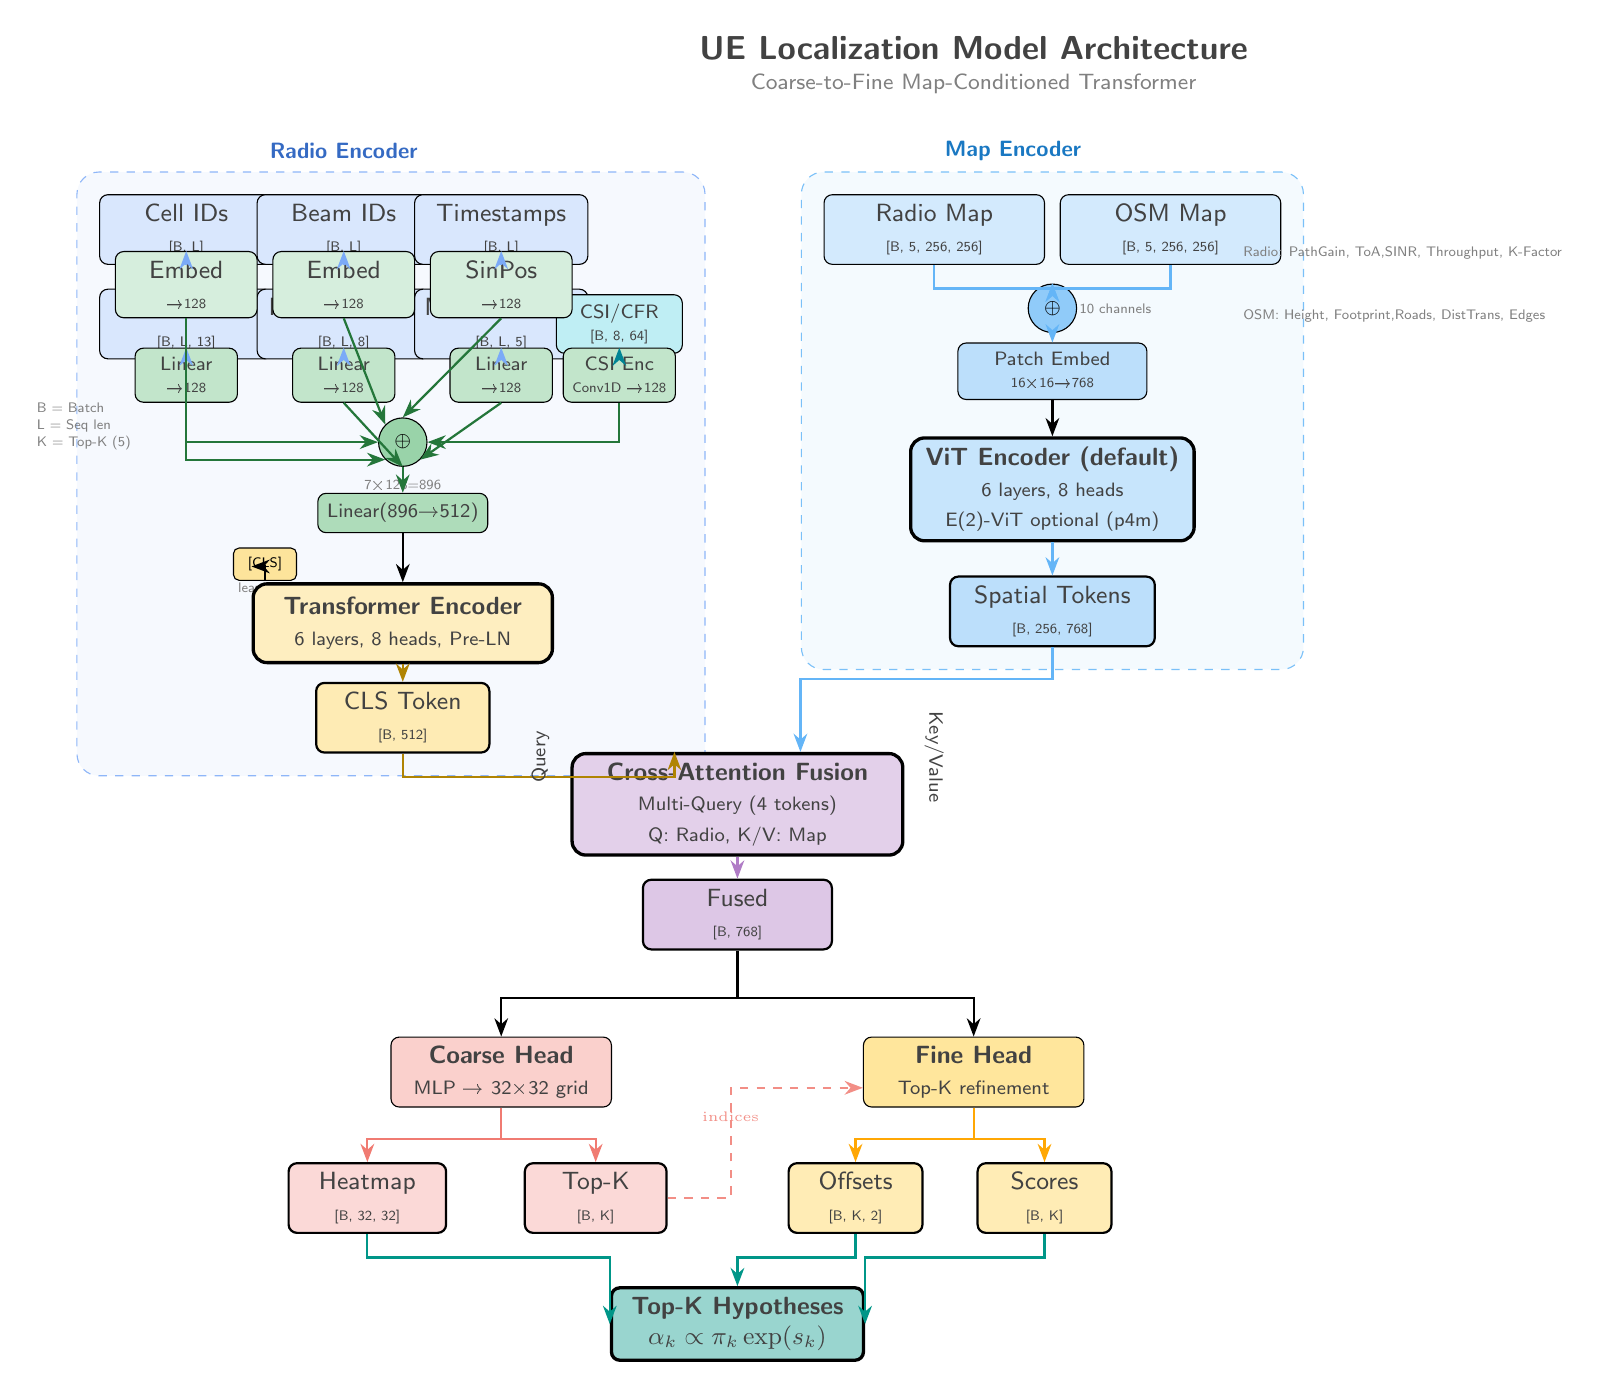
\begin{tikzpicture}[
    node distance=0.6cm and 0.8cm,
    >=Latex,
    font=\sffamily\small,
    % Block styles
    inputbox/.style={draw, rounded corners=3pt, fill=inputblue!20, minimum width=2.2cm, minimum height=0.7cm, align=center, text=darkgray},
    embedbox/.style={draw, rounded corners=3pt, fill=embedgreen!20, minimum width=1.8cm, minimum height=0.6cm, align=center, text=darkgray},
    projbox/.style={draw, rounded corners=3pt, fill=embedgreen!30, minimum width=1.3cm, minimum height=0.5cm, align=center, font=\sffamily\scriptsize, text=darkgray},
    transformer/.style={draw, rounded corners=5pt, fill=transformerorange!25, minimum width=3.2cm, minimum height=1.0cm, align=center, text=darkgray, very thick},
    fusionbox/.style={draw, rounded corners=5pt, fill=fusionpurple!25, minimum width=3.0cm, minimum height=0.9cm, align=center, text=darkgray, very thick},
    headbox/.style={draw, rounded corners=3pt, fill=coarsered!20, minimum width=2.8cm, minimum height=0.8cm, align=center, text=darkgray},
    outputbox/.style={draw, rounded corners=3pt, fill=outputteal!25, minimum width=2.4cm, minimum height=0.7cm, align=center, text=darkgray, thick},
    mapbox/.style={draw, rounded corners=3pt, fill=mapblue!20, minimum width=2.2cm, minimum height=0.7cm, align=center, text=darkgray},
    cfrbox/.style={draw, rounded corners=3pt, fill=cfrcyan!25, minimum width=1.6cm, minimum height=0.5cm, align=center, font=\sffamily\scriptsize, text=darkgray},
    arrow/.style={->, thick, >=Stealth},
    dasharrow/.style={->, thick, >=Stealth, dashed},
    catarrow/.style={->, thick, >=Stealth, color=embedgreen!70!black},
    label/.style={font=\sffamily\scriptsize, text=darkgray},
    dimtext/.style={font=\sffamily\tiny, text=gray},
]

% ============================================
% TITLE
% ============================================
\node[font=\sffamily\bfseries\large, text=darkgray] at (4.5, 8.8) {UE Localization Model Architecture};
\node[font=\sffamily\footnotesize, text=gray] at (4.5, 8.35) {Coarse-to-Fine Map-Conditioned Transformer};

% ============================================
% LEFT SIDE: RADIO ENCODER
% ============================================
\node[font=\sffamily\bfseries\footnotesize, text=inputblue!80!black] at (-3.5, 7.5) {Radio Encoder};

% Input Boxes
\node[inputbox] (cellin) at (-5.5, 6.5) {Cell IDs\\{\tiny [B, L]}};
\node[inputbox] (beamin) at (-3.5, 6.5) {Beam IDs\\{\tiny [B, L]}};
\node[inputbox] (timein) at (-1.5, 6.5) {Timestamps\\{\tiny [B, L]}};

\node[inputbox] (rtin) at (-5.5, 5.3) {RT Features\\{\tiny [B, L, 13]}};
\node[inputbox] (phyin) at (-3.5, 5.3) {PHY Features\\{\tiny [B, L, 8]}};
\node[inputbox] (macin) at (-1.5, 5.3) {MAC Features\\{\tiny [B, L, 5]}};

\node[cfrbox] (cfrin) at (-0.0, 5.3) {CSI/CFR\\{\tiny [B, 8, 64]}};

% Embedding/Projection layers
\node[embedbox] (cellemb) at (-5.5, 5.8) {Embed\\{\tiny →128}};
\node[embedbox] (beamemb) at (-3.5, 5.8) {Embed\\{\tiny →128}};
\node[embedbox] (timeemb) at (-1.5, 5.8) {SinPos\\{\tiny →128}};

\node[projbox] (rtproj) at (-5.5, 4.65) {Linear\\{\tiny →128}};
\node[projbox] (phyproj) at (-3.5, 4.65) {Linear\\{\tiny →128}};
\node[projbox] (macproj) at (-1.5, 4.65) {Linear\\{\tiny →128}};
\node[projbox] (cfrenc) at (0.0, 4.65) {CSI Enc\\{\tiny Conv1D →128}};

% Arrows from inputs to embeddings
\draw[arrow, inputblue!70] (cellin.south) -- (cellemb.north);
\draw[arrow, inputblue!70] (beamin.south) -- (beamemb.north);
\draw[arrow, inputblue!70] (timein.south) -- (timeemb.north);
\draw[arrow, inputblue!70] (rtin.south) -- (rtproj.north);
\draw[arrow, inputblue!70] (phyin.south) -- (phyproj.north);
\draw[arrow, inputblue!70] (macin.south) -- (macproj.north);
\draw[arrow, cfrcyan!70!black] (cfrin.south) -- (cfrenc.north);

% Concatenation node
\node[draw, circle, fill=embedgreen!50, minimum size=0.5cm, font=\sffamily\bfseries\scriptsize] (concat) at (-2.75, 3.8) {$\oplus$};
\node[dimtext, below=0.05cm of concat] {{\tiny 7×128=896}};

% Arrows to concatenation
\draw[catarrow] (cellemb.south) |- (concat.west);
\draw[catarrow] (beamemb.south) -- (concat.north west);
\draw[catarrow] (timeemb.south) -- (concat.north);
\draw[catarrow] (rtproj.south) |- (concat.south west);
\draw[catarrow] (phyproj.south) -- (concat.south);
\draw[catarrow] (macproj.south) -- (concat.south east);
\draw[catarrow] (cfrenc.south) |- (concat.east);

% Linear projection
\node[projbox, minimum width=2.0cm, fill=embedgreen!40] (inputproj) at (-2.75, 2.9) {Linear(896→512)};
\draw[arrow, embedgreen!70!black] (concat.south) -- (inputproj.north);

% CLS Token
\node[draw, rounded corners=2pt, fill=transformerorange!40, minimum width=0.8cm, minimum height=0.4cm, font=\sffamily\tiny] (cls) at (-4.5, 2.25) {[CLS]};
\node[dimtext] at (-4.5, 1.95) {{\tiny learnable}};

% Transformer Encoder
\node[transformer, minimum width=3.8cm] (radioenc) at (-2.75, 1.5) {\textbf{Transformer Encoder}\\{\scriptsize 6 layers, 8 heads, Pre-LN}};
\draw[arrow] (inputproj.south) -- ++(0, -0.25) -| (radioenc.north);
\draw[arrow] (cls.south) |- ([yshift=0.2cm]radioenc.north west);

% CLS output
\node[outputbox, fill=transformerorange!30, minimum width=2.2cm] (radiocls) at (-2.75, 0.3) {CLS Token\\{\tiny [B, 512]}};
\draw[arrow, transformerorange!70!black] (radioenc.south) -- (radiocls.north);

% ============================================
% RIGHT SIDE: MAP ENCODER
% ============================================
\node[font=\sffamily\bfseries\footnotesize, text=mapblue!80!black] at (5.0, 7.5) {Map Encoder};

% Map inputs
\node[mapbox, minimum width=2.8cm] (radiomap) at (4.0, 6.5) {Radio Map\\{\tiny [B, 5, 256, 256]}};
\node[mapbox, minimum width=2.8cm] (osmmap) at (7.0, 6.5) {OSM Map\\{\tiny [B, 5, 256, 256]}};

% Early fusion
\node[draw, circle, fill=mapblue!50, minimum size=0.5cm, font=\sffamily\bfseries\scriptsize] (mapconcat) at (5.5, 5.5) {$\oplus$};
\node[dimtext] at (6.3, 5.5) {{\tiny 10 channels}};
\draw[arrow, mapblue!70] (radiomap.south) -- ++(0, -0.3) -| (mapconcat);
\draw[arrow, mapblue!70] (osmmap.south) -- ++(0, -0.3) -| (mapconcat);

% Patch embedding
\node[projbox, minimum width=2.4cm, fill=mapblue!30] (patchemb) at (5.5, 4.7) {Patch Embed\\{\tiny 16×16→768}};
\draw[arrow, mapblue!70] (mapconcat.south) -- (patchemb.north);

% Map Vision Transformer
\node[transformer, minimum width=3.6cm, fill=mapblue!25] (mapvit) at (5.5, 3.2) {\textbf{ViT Encoder (default)}\\{\scriptsize 6 layers, 8 heads}\\{\scriptsize E(2)-ViT optional (p4m)}};
\draw[arrow] (patchemb.south) -- (mapvit.north);

% Map spatial tokens output
\node[outputbox, fill=mapblue!30, minimum width=2.6cm] (maptokens) at (5.5, 1.65) {Spatial Tokens\\{\tiny [B, 256, 768]}};
\draw[arrow, mapblue!70] (mapvit.south) -- (maptokens.north);

% ============================================
% CENTER: CROSS-ATTENTION FUSION
% ============================================
\node[fusionbox, minimum width=4.2cm, minimum height=1.2cm] (fusion) at (1.5, -0.8) {\textbf{Cross-Attention Fusion}\\{\scriptsize Multi-Query (4 tokens)}\\{\scriptsize Q: Radio, K/V: Map}};

% Arrows to fusion
\draw[arrow, transformerorange!70!black] (radiocls.south) -- ++(0, -0.3) -| ([xshift=-0.8cm]fusion.north);
\draw[arrow, mapblue!70] (maptokens.south) -- ++(0, -0.4) -| ([xshift=0.8cm]fusion.north);

% Labels
\node[label, rotate=90] at (-1.0, -0.2) {Query};
\node[label, rotate=-90] at (4.0, -0.2) {Key/Value};

% Fused output
\node[outputbox, fill=fusionpurple!30, minimum width=2.4cm] (fused) at (1.5, -2.2) {Fused\\{\tiny [B, 768]}};
\draw[arrow, fusionpurple!70] (fusion.south) -- (fused.north);

% ============================================
% BOTTOM: PREDICTION HEADS
% ============================================
% Coarse Head
\node[headbox, fill=coarsered!25] (coarse) at (-1.5, -4.2) {\textbf{Coarse Head}\\{\scriptsize MLP → 32×32 grid}};
\draw[arrow] (fused.south) -- ++(0, -0.6) -| (coarse.north);

% Fine Head
\node[headbox, fill=fineyellow!40] (fine) at (4.5, -4.2) {\textbf{Fine Head}\\{\scriptsize Top-K refinement}};
\draw[arrow] (fused.south) -- ++(0, -0.6) -| (fine.north);

% Coarse outputs
\node[outputbox, fill=coarsered!20, minimum width=2.0cm] (heatmap) at (-3.2, -5.8) {Heatmap\\{\tiny [B, 32, 32]}};
\node[outputbox, fill=coarsered!20, minimum width=1.8cm] (topk) at (-0.3, -5.8) {Top-K\\{\tiny [B, K]}};
\draw[arrow, coarsered!70] (coarse.south) -- ++(0, -0.4) -| (heatmap.north);
\draw[arrow, coarsered!70] (coarse.south) -- ++(0, -0.4) -| (topk.north);

% Connection from coarse to fine (top-k indices)
\draw[dasharrow, coarsered!60] (topk.east) -- ++(0.8, 0) |- ([yshift=-0.2cm]fine.west) node[pos=0.3, above, font=\tiny] {indices};

% Fine outputs
\node[outputbox, fill=fineyellow!30, minimum width=1.7cm] (offsets) at (3.0, -5.8) {Offsets\\{\tiny [B, K, 2]}};
\node[outputbox, fill=fineyellow!30, minimum width=1.7cm] (scores) at (5.4, -5.8) {Scores\\{\tiny [B, K]}};
\draw[arrow, fineyellow!60!orange] (fine.south) -- ++(0, -0.4) -| (offsets.north);
\draw[arrow, fineyellow!60!orange] (fine.south) -- ++(0, -0.4) -| (scores.north);

% ============================================
% FINAL OUTPUT
% ============================================
\node[outputbox, fill=outputteal!40, minimum width=3.2cm, minimum height=0.8cm, very thick] (finalpos) at (1.5, -7.4) {\textbf{Top-K Hypotheses}\\$\alpha_k \propto \pi_k \exp(s_k)$};
\draw[arrow, thick, outputteal] (heatmap.south) |- ++(0, -0.3) -| (finalpos.west);
\draw[arrow, thick, outputteal] (offsets.south) |- ++(0, -0.3) -| (finalpos);
\draw[arrow, thick, outputteal] (scores.south) |- ++(0, -0.3) -| (finalpos.east);

% ============================================
% ANNOTATIONS/LEGEND
% ============================================
% Dashed box around radio encoder
\begin{scope}[on background layer]
    \node[draw=inputblue!60, dashed, rounded corners=8pt, fit=(cellin)(cfrin)(radioenc)(radiocls), inner sep=8pt, fill=inputblue!5] {};
\end{scope}

% Dashed box around map encoder  
\begin{scope}[on background layer]
    \node[draw=mapblue!60, dashed, rounded corners=8pt, fit=(radiomap)(osmmap)(mapvit)(maptokens), inner sep=8pt, fill=mapblue!5] {};
\end{scope}

% Dimension annotations
\node[font=\sffamily\tiny, text=gray, align=left] at (-6.8, 4.0) {B = Batch\\L = Seq len\\K = Top-K (5)};

% Channel annotations for maps
\node[font=\sffamily\tiny, text=gray, right] at (7.8, 6.2) {Radio: PathGain, ToA,\\SINR, Throughput, K-Factor};
\node[font=\sffamily\tiny, text=gray, right] at (7.8, 5.4) {OSM: Height, Footprint,\\Roads, DistTrans, Edges};

\end{tikzpicture}
\end{document}


\documentclass[border=5pt]{standalone}
\usepackage{tikz}
\usetikzlibrary{positioning, arrows.meta, shapes.geometric, fit, calc, backgrounds, decorations.pathreplacing, patterns}
\usepackage{amsmath}
\usepackage{xcolor}

% Define colors matching the implementation
\definecolor{inputblue}{RGB}{66, 133, 244}
\definecolor{embedgreen}{RGB}{52, 168, 83}
\definecolor{transformerorange}{RGB}{251, 188, 5}
\definecolor{fusionpurple}{RGB}{142, 68, 173}
\definecolor{coarsered}{RGB}{234, 67, 53}
\definecolor{fineyellow}{RGB}{255, 193, 7}
\definecolor{outputteal}{RGB}{0, 150, 136}
\definecolor{mapblue}{RGB}{33, 150, 243}
\definecolor{cfrcyan}{RGB}{0, 188, 212}
\definecolor{lightgray}{RGB}{245, 245, 245}
\definecolor{darkgray}{RGB}{66, 66, 66}

\begin{document}
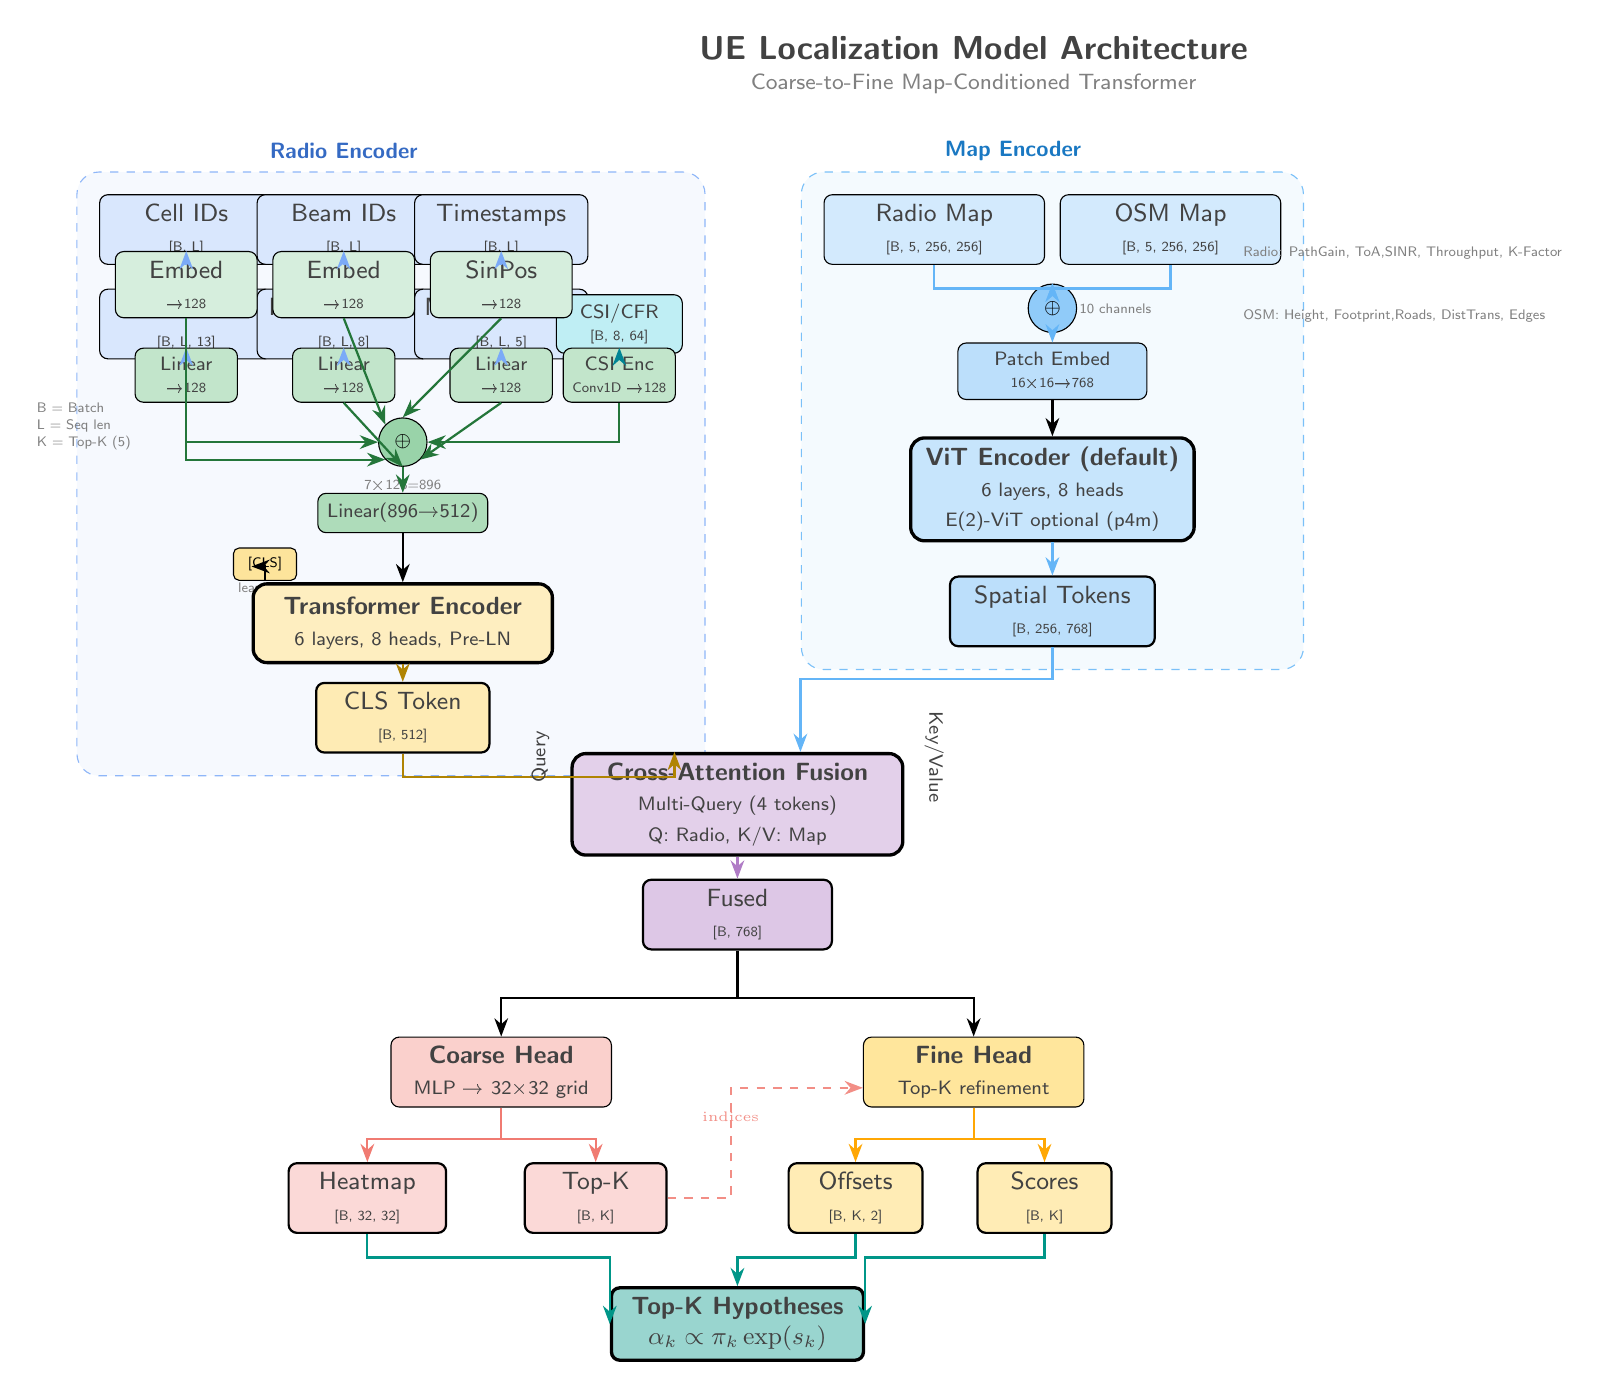
\begin{tikzpicture}[
    node distance=0.6cm and 0.8cm,
    >=Latex,
    font=\sffamily\small,
    % Block styles
    inputbox/.style={draw, rounded corners=3pt, fill=inputblue!20, minimum width=2.2cm, minimum height=0.7cm, align=center, text=darkgray},
    embedbox/.style={draw, rounded corners=3pt, fill=embedgreen!20, minimum width=1.8cm, minimum height=0.6cm, align=center, text=darkgray},
    projbox/.style={draw, rounded corners=3pt, fill=embedgreen!30, minimum width=1.3cm, minimum height=0.5cm, align=center, font=\sffamily\scriptsize, text=darkgray},
    transformer/.style={draw, rounded corners=5pt, fill=transformerorange!25, minimum width=3.2cm, minimum height=1.0cm, align=center, text=darkgray, very thick},
    fusionbox/.style={draw, rounded corners=5pt, fill=fusionpurple!25, minimum width=3.0cm, minimum height=0.9cm, align=center, text=darkgray, very thick},
    headbox/.style={draw, rounded corners=3pt, fill=coarsered!20, minimum width=2.8cm, minimum height=0.8cm, align=center, text=darkgray},
    outputbox/.style={draw, rounded corners=3pt, fill=outputteal!25, minimum width=2.4cm, minimum height=0.7cm, align=center, text=darkgray, thick},
    mapbox/.style={draw, rounded corners=3pt, fill=mapblue!20, minimum width=2.2cm, minimum height=0.7cm, align=center, text=darkgray},
    cfrbox/.style={draw, rounded corners=3pt, fill=cfrcyan!25, minimum width=1.6cm, minimum height=0.5cm, align=center, font=\sffamily\scriptsize, text=darkgray},
    arrow/.style={->, thick, >=Stealth},
    dasharrow/.style={->, thick, >=Stealth, dashed},
    catarrow/.style={->, thick, >=Stealth, color=embedgreen!70!black},
    label/.style={font=\sffamily\scriptsize, text=darkgray},
    dimtext/.style={font=\sffamily\tiny, text=gray},
]

% ============================================
% TITLE
% ============================================
\node[font=\sffamily\bfseries\large, text=darkgray] at (4.5, 8.8) {UE Localization Model Architecture};
\node[font=\sffamily\footnotesize, text=gray] at (4.5, 8.35) {Coarse-to-Fine Map-Conditioned Transformer};

% ============================================
% LEFT SIDE: RADIO ENCODER
% ============================================
\node[font=\sffamily\bfseries\footnotesize, text=inputblue!80!black] at (-3.5, 7.5) {Radio Encoder};

% Input Boxes
\node[inputbox] (cellin) at (-5.5, 6.5) {Cell IDs\\{\tiny [B, L]}};
\node[inputbox] (beamin) at (-3.5, 6.5) {Beam IDs\\{\tiny [B, L]}};
\node[inputbox] (timein) at (-1.5, 6.5) {Timestamps\\{\tiny [B, L]}};

\node[inputbox] (rtin) at (-5.5, 5.3) {RT Features\\{\tiny [B, L, 13]}};
\node[inputbox] (phyin) at (-3.5, 5.3) {PHY Features\\{\tiny [B, L, 8]}};
\node[inputbox] (macin) at (-1.5, 5.3) {MAC Features\\{\tiny [B, L, 5]}};

\node[cfrbox] (cfrin) at (-0.0, 5.3) {CSI/CFR\\{\tiny [B, 8, 64]}};

% Embedding/Projection layers
\node[embedbox] (cellemb) at (-5.5, 5.8) {Embed\\{\tiny →128}};
\node[embedbox] (beamemb) at (-3.5, 5.8) {Embed\\{\tiny →128}};
\node[embedbox] (timeemb) at (-1.5, 5.8) {SinPos\\{\tiny →128}};

\node[projbox] (rtproj) at (-5.5, 4.65) {Linear\\{\tiny →128}};
\node[projbox] (phyproj) at (-3.5, 4.65) {Linear\\{\tiny →128}};
\node[projbox] (macproj) at (-1.5, 4.65) {Linear\\{\tiny →128}};
\node[projbox] (cfrenc) at (0.0, 4.65) {CSI Enc\\{\tiny Conv1D →128}};

% Arrows from inputs to embeddings
\draw[arrow, inputblue!70] (cellin.south) -- (cellemb.north);
\draw[arrow, inputblue!70] (beamin.south) -- (beamemb.north);
\draw[arrow, inputblue!70] (timein.south) -- (timeemb.north);
\draw[arrow, inputblue!70] (rtin.south) -- (rtproj.north);
\draw[arrow, inputblue!70] (phyin.south) -- (phyproj.north);
\draw[arrow, inputblue!70] (macin.south) -- (macproj.north);
\draw[arrow, cfrcyan!70!black] (cfrin.south) -- (cfrenc.north);

% Concatenation node
\node[draw, circle, fill=embedgreen!50, minimum size=0.5cm, font=\sffamily\bfseries\scriptsize] (concat) at (-2.75, 3.8) {$\oplus$};
\node[dimtext, below=0.05cm of concat] {{\tiny 7×128=896}};

% Arrows to concatenation
\draw[catarrow] (cellemb.south) |- (concat.west);
\draw[catarrow] (beamemb.south) -- (concat.north west);
\draw[catarrow] (timeemb.south) -- (concat.north);
\draw[catarrow] (rtproj.south) |- (concat.south west);
\draw[catarrow] (phyproj.south) -- (concat.south);
\draw[catarrow] (macproj.south) -- (concat.south east);
\draw[catarrow] (cfrenc.south) |- (concat.east);

% Linear projection
\node[projbox, minimum width=2.0cm, fill=embedgreen!40] (inputproj) at (-2.75, 2.9) {Linear(896→512)};
\draw[arrow, embedgreen!70!black] (concat.south) -- (inputproj.north);

% CLS Token
\node[draw, rounded corners=2pt, fill=transformerorange!40, minimum width=0.8cm, minimum height=0.4cm, font=\sffamily\tiny] (cls) at (-4.5, 2.25) {[CLS]};
\node[dimtext] at (-4.5, 1.95) {{\tiny learnable}};

% Transformer Encoder
\node[transformer, minimum width=3.8cm] (radioenc) at (-2.75, 1.5) {\textbf{Transformer Encoder}\\{\scriptsize 6 layers, 8 heads, Pre-LN}};
\draw[arrow] (inputproj.south) -- ++(0, -0.25) -| (radioenc.north);
\draw[arrow] (cls.south) |- ([yshift=0.2cm]radioenc.north west);

% CLS output
\node[outputbox, fill=transformerorange!30, minimum width=2.2cm] (radiocls) at (-2.75, 0.3) {CLS Token\\{\tiny [B, 512]}};
\draw[arrow, transformerorange!70!black] (radioenc.south) -- (radiocls.north);

% ============================================
% RIGHT SIDE: MAP ENCODER
% ============================================
\node[font=\sffamily\bfseries\footnotesize, text=mapblue!80!black] at (5.0, 7.5) {Map Encoder};

% Map inputs
\node[mapbox, minimum width=2.8cm] (radiomap) at (4.0, 6.5) {Radio Map\\{\tiny [B, 5, 256, 256]}};
\node[mapbox, minimum width=2.8cm] (osmmap) at (7.0, 6.5) {OSM Map\\{\tiny [B, 5, 256, 256]}};

% Early fusion
\node[draw, circle, fill=mapblue!50, minimum size=0.5cm, font=\sffamily\bfseries\scriptsize] (mapconcat) at (5.5, 5.5) {$\oplus$};
\node[dimtext] at (6.3, 5.5) {{\tiny 10 channels}};
\draw[arrow, mapblue!70] (radiomap.south) -- ++(0, -0.3) -| (mapconcat);
\draw[arrow, mapblue!70] (osmmap.south) -- ++(0, -0.3) -| (mapconcat);

% Patch embedding
\node[projbox, minimum width=2.4cm, fill=mapblue!30] (patchemb) at (5.5, 4.7) {Patch Embed\\{\tiny 16×16→768}};
\draw[arrow, mapblue!70] (mapconcat.south) -- (patchemb.north);

% Map Vision Transformer
\node[transformer, minimum width=3.6cm, fill=mapblue!25] (mapvit) at (5.5, 3.2) {\textbf{ViT Encoder (default)}\\{\scriptsize 6 layers, 8 heads}\\{\scriptsize E(2)-ViT optional (p4m)}};
\draw[arrow] (patchemb.south) -- (mapvit.north);

% Map spatial tokens output
\node[outputbox, fill=mapblue!30, minimum width=2.6cm] (maptokens) at (5.5, 1.65) {Spatial Tokens\\{\tiny [B, 256, 768]}};
\draw[arrow, mapblue!70] (mapvit.south) -- (maptokens.north);

% ============================================
% CENTER: CROSS-ATTENTION FUSION
% ============================================
\node[fusionbox, minimum width=4.2cm, minimum height=1.2cm] (fusion) at (1.5, -0.8) {\textbf{Cross-Attention Fusion}\\{\scriptsize Multi-Query (4 tokens)}\\{\scriptsize Q: Radio, K/V: Map}};

% Arrows to fusion
\draw[arrow, transformerorange!70!black] (radiocls.south) -- ++(0, -0.3) -| ([xshift=-0.8cm]fusion.north);
\draw[arrow, mapblue!70] (maptokens.south) -- ++(0, -0.4) -| ([xshift=0.8cm]fusion.north);

% Labels
\node[label, rotate=90] at (-1.0, -0.2) {Query};
\node[label, rotate=-90] at (4.0, -0.2) {Key/Value};

% Fused output
\node[outputbox, fill=fusionpurple!30, minimum width=2.4cm] (fused) at (1.5, -2.2) {Fused\\{\tiny [B, 768]}};
\draw[arrow, fusionpurple!70] (fusion.south) -- (fused.north);

% ============================================
% BOTTOM: PREDICTION HEADS
% ============================================
% Coarse Head
\node[headbox, fill=coarsered!25] (coarse) at (-1.5, -4.2) {\textbf{Coarse Head}\\{\scriptsize MLP → 32×32 grid}};
\draw[arrow] (fused.south) -- ++(0, -0.6) -| (coarse.north);

% Fine Head
\node[headbox, fill=fineyellow!40] (fine) at (4.5, -4.2) {\textbf{Fine Head}\\{\scriptsize Top-K refinement}};
\draw[arrow] (fused.south) -- ++(0, -0.6) -| (fine.north);

% Coarse outputs
\node[outputbox, fill=coarsered!20, minimum width=2.0cm] (heatmap) at (-3.2, -5.8) {Heatmap\\{\tiny [B, 32, 32]}};
\node[outputbox, fill=coarsered!20, minimum width=1.8cm] (topk) at (-0.3, -5.8) {Top-K\\{\tiny [B, K]}};
\draw[arrow, coarsered!70] (coarse.south) -- ++(0, -0.4) -| (heatmap.north);
\draw[arrow, coarsered!70] (coarse.south) -- ++(0, -0.4) -| (topk.north);

% Connection from coarse to fine (top-k indices)
\draw[dasharrow, coarsered!60] (topk.east) -- ++(0.8, 0) |- ([yshift=-0.2cm]fine.west) node[pos=0.3, above, font=\tiny] {indices};

% Fine outputs
\node[outputbox, fill=fineyellow!30, minimum width=1.7cm] (offsets) at (3.0, -5.8) {Offsets\\{\tiny [B, K, 2]}};
\node[outputbox, fill=fineyellow!30, minimum width=1.7cm] (scores) at (5.4, -5.8) {Scores\\{\tiny [B, K]}};
\draw[arrow, fineyellow!60!orange] (fine.south) -- ++(0, -0.4) -| (offsets.north);
\draw[arrow, fineyellow!60!orange] (fine.south) -- ++(0, -0.4) -| (scores.north);

% ============================================
% FINAL OUTPUT
% ============================================
\node[outputbox, fill=outputteal!40, minimum width=3.2cm, minimum height=0.8cm, very thick] (finalpos) at (1.5, -7.4) {\textbf{Top-K Hypotheses}\\$\alpha_k \propto \pi_k \exp(s_k)$};
\draw[arrow, thick, outputteal] (heatmap.south) |- ++(0, -0.3) -| (finalpos.west);
\draw[arrow, thick, outputteal] (offsets.south) |- ++(0, -0.3) -| (finalpos);
\draw[arrow, thick, outputteal] (scores.south) |- ++(0, -0.3) -| (finalpos.east);

% ============================================
% ANNOTATIONS/LEGEND
% ============================================
% Dashed box around radio encoder
\begin{scope}[on background layer]
    \node[draw=inputblue!60, dashed, rounded corners=8pt, fit=(cellin)(cfrin)(radioenc)(radiocls), inner sep=8pt, fill=inputblue!5] {};
\end{scope}

% Dashed box around map encoder  
\begin{scope}[on background layer]
    \node[draw=mapblue!60, dashed, rounded corners=8pt, fit=(radiomap)(osmmap)(mapvit)(maptokens), inner sep=8pt, fill=mapblue!5] {};
\end{scope}

% Dimension annotations
\node[font=\sffamily\tiny, text=gray, align=left] at (-6.8, 4.0) {B = Batch\\L = Seq len\\K = Top-K (5)};

% Channel annotations for maps
\node[font=\sffamily\tiny, text=gray, right] at (7.8, 6.2) {Radio: PathGain, ToA,\\SINR, Throughput, K-Factor};
\node[font=\sffamily\tiny, text=gray, right] at (7.8, 5.4) {OSM: Height, Footprint,\\Roads, DistTrans, Edges};

\end{tikzpicture}
\end{document}


\documentclass[border=5pt]{standalone}
\usepackage{tikz}
\usetikzlibrary{positioning, arrows.meta, shapes.geometric, fit, calc, backgrounds, decorations.pathreplacing, patterns}
\usepackage{amsmath}
\usepackage{xcolor}

% Define colors matching the implementation
\definecolor{inputblue}{RGB}{66, 133, 244}
\definecolor{embedgreen}{RGB}{52, 168, 83}
\definecolor{transformerorange}{RGB}{251, 188, 5}
\definecolor{fusionpurple}{RGB}{142, 68, 173}
\definecolor{coarsered}{RGB}{234, 67, 53}
\definecolor{fineyellow}{RGB}{255, 193, 7}
\definecolor{outputteal}{RGB}{0, 150, 136}
\definecolor{mapblue}{RGB}{33, 150, 243}
\definecolor{cfrcyan}{RGB}{0, 188, 212}
\definecolor{lightgray}{RGB}{245, 245, 245}
\definecolor{darkgray}{RGB}{66, 66, 66}

\begin{document}
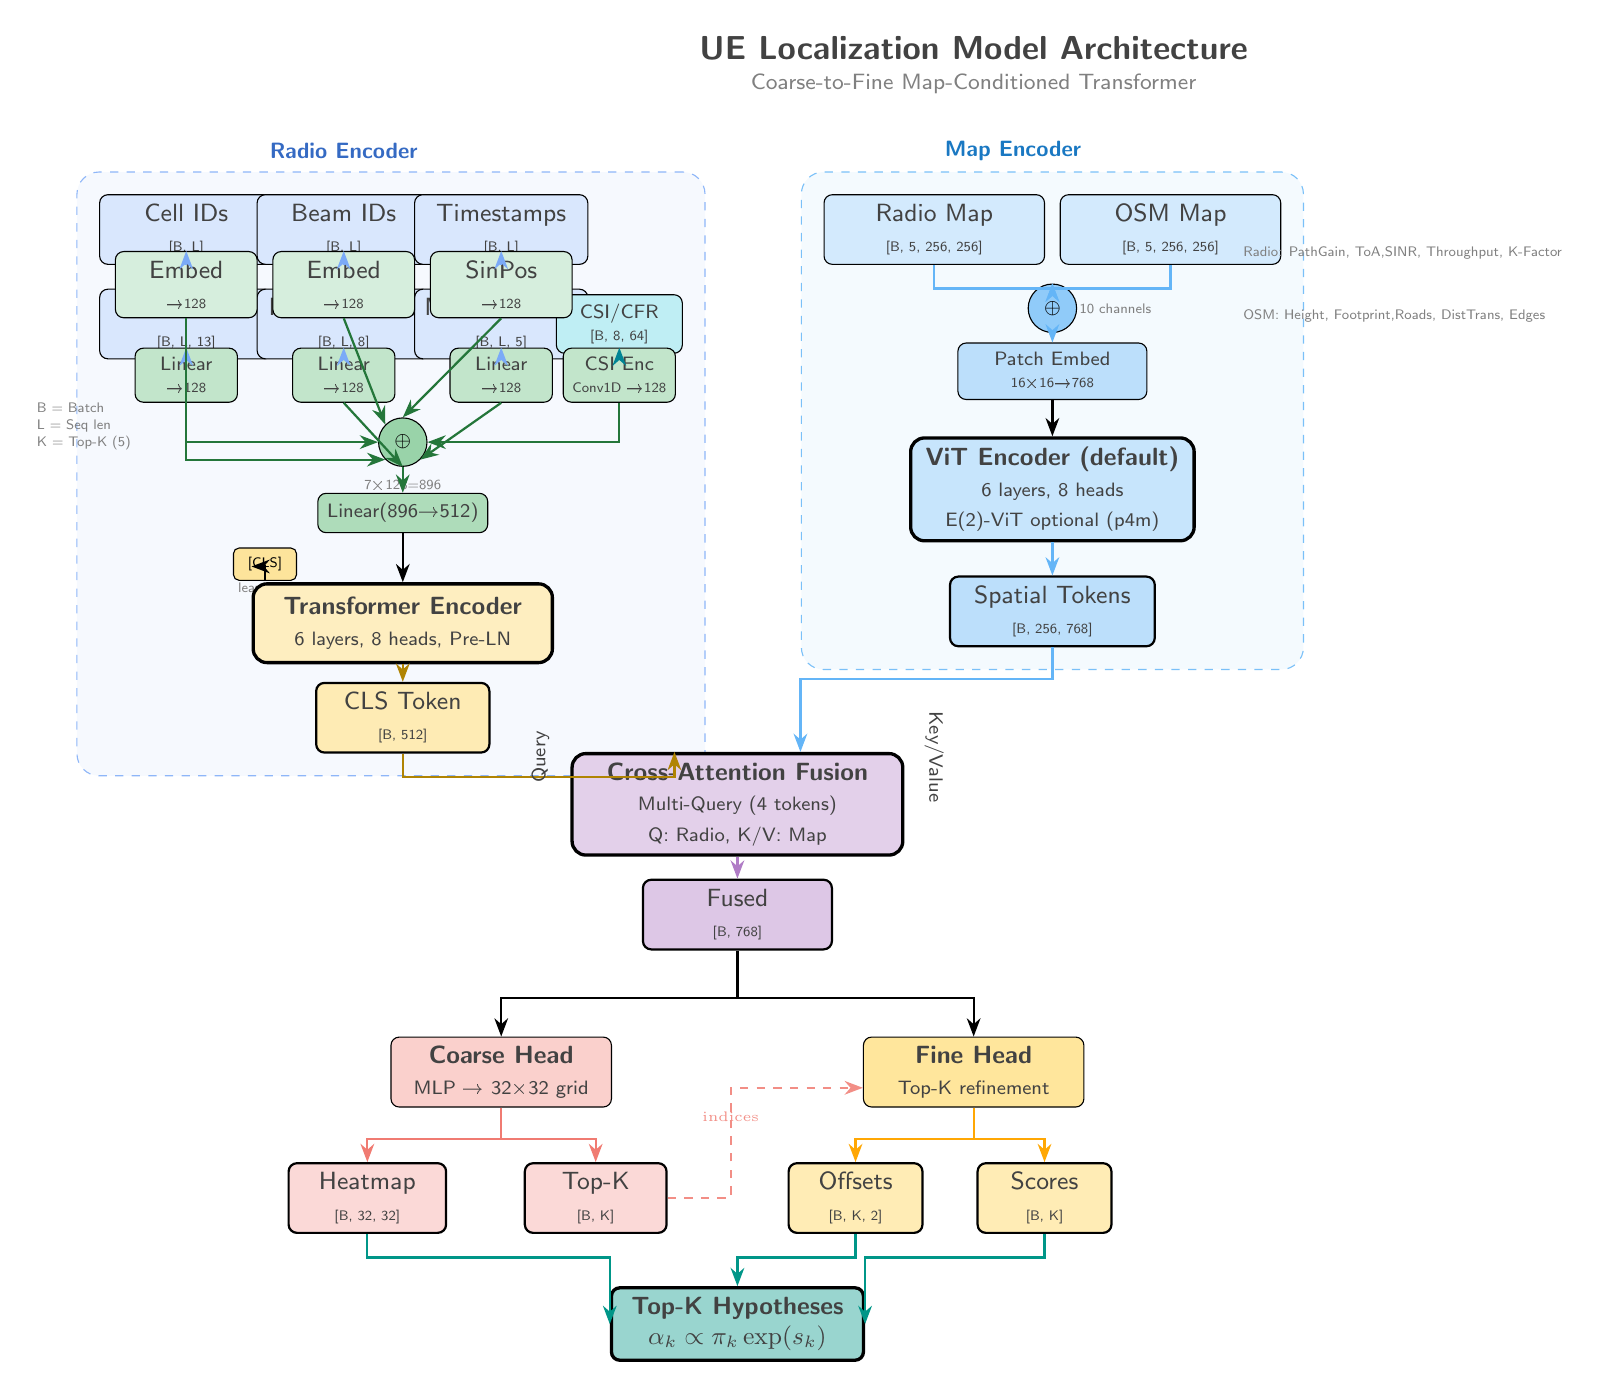
\begin{tikzpicture}[
    node distance=0.6cm and 0.8cm,
    >=Latex,
    font=\sffamily\small,
    % Block styles
    inputbox/.style={draw, rounded corners=3pt, fill=inputblue!20, minimum width=2.2cm, minimum height=0.7cm, align=center, text=darkgray},
    embedbox/.style={draw, rounded corners=3pt, fill=embedgreen!20, minimum width=1.8cm, minimum height=0.6cm, align=center, text=darkgray},
    projbox/.style={draw, rounded corners=3pt, fill=embedgreen!30, minimum width=1.3cm, minimum height=0.5cm, align=center, font=\sffamily\scriptsize, text=darkgray},
    transformer/.style={draw, rounded corners=5pt, fill=transformerorange!25, minimum width=3.2cm, minimum height=1.0cm, align=center, text=darkgray, very thick},
    fusionbox/.style={draw, rounded corners=5pt, fill=fusionpurple!25, minimum width=3.0cm, minimum height=0.9cm, align=center, text=darkgray, very thick},
    headbox/.style={draw, rounded corners=3pt, fill=coarsered!20, minimum width=2.8cm, minimum height=0.8cm, align=center, text=darkgray},
    outputbox/.style={draw, rounded corners=3pt, fill=outputteal!25, minimum width=2.4cm, minimum height=0.7cm, align=center, text=darkgray, thick},
    mapbox/.style={draw, rounded corners=3pt, fill=mapblue!20, minimum width=2.2cm, minimum height=0.7cm, align=center, text=darkgray},
    cfrbox/.style={draw, rounded corners=3pt, fill=cfrcyan!25, minimum width=1.6cm, minimum height=0.5cm, align=center, font=\sffamily\scriptsize, text=darkgray},
    arrow/.style={->, thick, >=Stealth},
    dasharrow/.style={->, thick, >=Stealth, dashed},
    catarrow/.style={->, thick, >=Stealth, color=embedgreen!70!black},
    label/.style={font=\sffamily\scriptsize, text=darkgray},
    dimtext/.style={font=\sffamily\tiny, text=gray},
]

% ============================================
% TITLE
% ============================================
\node[font=\sffamily\bfseries\large, text=darkgray] at (4.5, 8.8) {UE Localization Model Architecture};
\node[font=\sffamily\footnotesize, text=gray] at (4.5, 8.35) {Coarse-to-Fine Map-Conditioned Transformer};

% ============================================
% LEFT SIDE: RADIO ENCODER
% ============================================
\node[font=\sffamily\bfseries\footnotesize, text=inputblue!80!black] at (-3.5, 7.5) {Radio Encoder};

% Input Boxes
\node[inputbox] (cellin) at (-5.5, 6.5) {Cell IDs\\{\tiny [B, L]}};
\node[inputbox] (beamin) at (-3.5, 6.5) {Beam IDs\\{\tiny [B, L]}};
\node[inputbox] (timein) at (-1.5, 6.5) {Timestamps\\{\tiny [B, L]}};

\node[inputbox] (rtin) at (-5.5, 5.3) {RT Features\\{\tiny [B, L, 13]}};
\node[inputbox] (phyin) at (-3.5, 5.3) {PHY Features\\{\tiny [B, L, 8]}};
\node[inputbox] (macin) at (-1.5, 5.3) {MAC Features\\{\tiny [B, L, 5]}};

\node[cfrbox] (cfrin) at (-0.0, 5.3) {CSI/CFR\\{\tiny [B, 8, 64]}};

% Embedding/Projection layers
\node[embedbox] (cellemb) at (-5.5, 5.8) {Embed\\{\tiny →128}};
\node[embedbox] (beamemb) at (-3.5, 5.8) {Embed\\{\tiny →128}};
\node[embedbox] (timeemb) at (-1.5, 5.8) {SinPos\\{\tiny →128}};

\node[projbox] (rtproj) at (-5.5, 4.65) {Linear\\{\tiny →128}};
\node[projbox] (phyproj) at (-3.5, 4.65) {Linear\\{\tiny →128}};
\node[projbox] (macproj) at (-1.5, 4.65) {Linear\\{\tiny →128}};
\node[projbox] (cfrenc) at (0.0, 4.65) {CSI Enc\\{\tiny Conv1D →128}};

% Arrows from inputs to embeddings
\draw[arrow, inputblue!70] (cellin.south) -- (cellemb.north);
\draw[arrow, inputblue!70] (beamin.south) -- (beamemb.north);
\draw[arrow, inputblue!70] (timein.south) -- (timeemb.north);
\draw[arrow, inputblue!70] (rtin.south) -- (rtproj.north);
\draw[arrow, inputblue!70] (phyin.south) -- (phyproj.north);
\draw[arrow, inputblue!70] (macin.south) -- (macproj.north);
\draw[arrow, cfrcyan!70!black] (cfrin.south) -- (cfrenc.north);

% Concatenation node
\node[draw, circle, fill=embedgreen!50, minimum size=0.5cm, font=\sffamily\bfseries\scriptsize] (concat) at (-2.75, 3.8) {$\oplus$};
\node[dimtext, below=0.05cm of concat] {{\tiny 7×128=896}};

% Arrows to concatenation
\draw[catarrow] (cellemb.south) |- (concat.west);
\draw[catarrow] (beamemb.south) -- (concat.north west);
\draw[catarrow] (timeemb.south) -- (concat.north);
\draw[catarrow] (rtproj.south) |- (concat.south west);
\draw[catarrow] (phyproj.south) -- (concat.south);
\draw[catarrow] (macproj.south) -- (concat.south east);
\draw[catarrow] (cfrenc.south) |- (concat.east);

% Linear projection
\node[projbox, minimum width=2.0cm, fill=embedgreen!40] (inputproj) at (-2.75, 2.9) {Linear(896→512)};
\draw[arrow, embedgreen!70!black] (concat.south) -- (inputproj.north);

% CLS Token
\node[draw, rounded corners=2pt, fill=transformerorange!40, minimum width=0.8cm, minimum height=0.4cm, font=\sffamily\tiny] (cls) at (-4.5, 2.25) {[CLS]};
\node[dimtext] at (-4.5, 1.95) {{\tiny learnable}};

% Transformer Encoder
\node[transformer, minimum width=3.8cm] (radioenc) at (-2.75, 1.5) {\textbf{Transformer Encoder}\\{\scriptsize 6 layers, 8 heads, Pre-LN}};
\draw[arrow] (inputproj.south) -- ++(0, -0.25) -| (radioenc.north);
\draw[arrow] (cls.south) |- ([yshift=0.2cm]radioenc.north west);

% CLS output
\node[outputbox, fill=transformerorange!30, minimum width=2.2cm] (radiocls) at (-2.75, 0.3) {CLS Token\\{\tiny [B, 512]}};
\draw[arrow, transformerorange!70!black] (radioenc.south) -- (radiocls.north);

% ============================================
% RIGHT SIDE: MAP ENCODER
% ============================================
\node[font=\sffamily\bfseries\footnotesize, text=mapblue!80!black] at (5.0, 7.5) {Map Encoder};

% Map inputs
\node[mapbox, minimum width=2.8cm] (radiomap) at (4.0, 6.5) {Radio Map\\{\tiny [B, 5, 256, 256]}};
\node[mapbox, minimum width=2.8cm] (osmmap) at (7.0, 6.5) {OSM Map\\{\tiny [B, 5, 256, 256]}};

% Early fusion
\node[draw, circle, fill=mapblue!50, minimum size=0.5cm, font=\sffamily\bfseries\scriptsize] (mapconcat) at (5.5, 5.5) {$\oplus$};
\node[dimtext] at (6.3, 5.5) {{\tiny 10 channels}};
\draw[arrow, mapblue!70] (radiomap.south) -- ++(0, -0.3) -| (mapconcat);
\draw[arrow, mapblue!70] (osmmap.south) -- ++(0, -0.3) -| (mapconcat);

% Patch embedding
\node[projbox, minimum width=2.4cm, fill=mapblue!30] (patchemb) at (5.5, 4.7) {Patch Embed\\{\tiny 16×16→768}};
\draw[arrow, mapblue!70] (mapconcat.south) -- (patchemb.north);

% Map Vision Transformer
\node[transformer, minimum width=3.6cm, fill=mapblue!25] (mapvit) at (5.5, 3.2) {\textbf{ViT Encoder (default)}\\{\scriptsize 6 layers, 8 heads}\\{\scriptsize E(2)-ViT optional (p4m)}};
\draw[arrow] (patchemb.south) -- (mapvit.north);

% Map spatial tokens output
\node[outputbox, fill=mapblue!30, minimum width=2.6cm] (maptokens) at (5.5, 1.65) {Spatial Tokens\\{\tiny [B, 256, 768]}};
\draw[arrow, mapblue!70] (mapvit.south) -- (maptokens.north);

% ============================================
% CENTER: CROSS-ATTENTION FUSION
% ============================================
\node[fusionbox, minimum width=4.2cm, minimum height=1.2cm] (fusion) at (1.5, -0.8) {\textbf{Cross-Attention Fusion}\\{\scriptsize Multi-Query (4 tokens)}\\{\scriptsize Q: Radio, K/V: Map}};

% Arrows to fusion
\draw[arrow, transformerorange!70!black] (radiocls.south) -- ++(0, -0.3) -| ([xshift=-0.8cm]fusion.north);
\draw[arrow, mapblue!70] (maptokens.south) -- ++(0, -0.4) -| ([xshift=0.8cm]fusion.north);

% Labels
\node[label, rotate=90] at (-1.0, -0.2) {Query};
\node[label, rotate=-90] at (4.0, -0.2) {Key/Value};

% Fused output
\node[outputbox, fill=fusionpurple!30, minimum width=2.4cm] (fused) at (1.5, -2.2) {Fused\\{\tiny [B, 768]}};
\draw[arrow, fusionpurple!70] (fusion.south) -- (fused.north);

% ============================================
% BOTTOM: PREDICTION HEADS
% ============================================
% Coarse Head
\node[headbox, fill=coarsered!25] (coarse) at (-1.5, -4.2) {\textbf{Coarse Head}\\{\scriptsize MLP → 32×32 grid}};
\draw[arrow] (fused.south) -- ++(0, -0.6) -| (coarse.north);

% Fine Head
\node[headbox, fill=fineyellow!40] (fine) at (4.5, -4.2) {\textbf{Fine Head}\\{\scriptsize Top-K refinement}};
\draw[arrow] (fused.south) -- ++(0, -0.6) -| (fine.north);

% Coarse outputs
\node[outputbox, fill=coarsered!20, minimum width=2.0cm] (heatmap) at (-3.2, -5.8) {Heatmap\\{\tiny [B, 32, 32]}};
\node[outputbox, fill=coarsered!20, minimum width=1.8cm] (topk) at (-0.3, -5.8) {Top-K\\{\tiny [B, K]}};
\draw[arrow, coarsered!70] (coarse.south) -- ++(0, -0.4) -| (heatmap.north);
\draw[arrow, coarsered!70] (coarse.south) -- ++(0, -0.4) -| (topk.north);

% Connection from coarse to fine (top-k indices)
\draw[dasharrow, coarsered!60] (topk.east) -- ++(0.8, 0) |- ([yshift=-0.2cm]fine.west) node[pos=0.3, above, font=\tiny] {indices};

% Fine outputs
\node[outputbox, fill=fineyellow!30, minimum width=1.7cm] (offsets) at (3.0, -5.8) {Offsets\\{\tiny [B, K, 2]}};
\node[outputbox, fill=fineyellow!30, minimum width=1.7cm] (scores) at (5.4, -5.8) {Scores\\{\tiny [B, K]}};
\draw[arrow, fineyellow!60!orange] (fine.south) -- ++(0, -0.4) -| (offsets.north);
\draw[arrow, fineyellow!60!orange] (fine.south) -- ++(0, -0.4) -| (scores.north);

% ============================================
% FINAL OUTPUT
% ============================================
\node[outputbox, fill=outputteal!40, minimum width=3.2cm, minimum height=0.8cm, very thick] (finalpos) at (1.5, -7.4) {\textbf{Top-K Hypotheses}\\$\alpha_k \propto \pi_k \exp(s_k)$};
\draw[arrow, thick, outputteal] (heatmap.south) |- ++(0, -0.3) -| (finalpos.west);
\draw[arrow, thick, outputteal] (offsets.south) |- ++(0, -0.3) -| (finalpos);
\draw[arrow, thick, outputteal] (scores.south) |- ++(0, -0.3) -| (finalpos.east);

% ============================================
% ANNOTATIONS/LEGEND
% ============================================
% Dashed box around radio encoder
\begin{scope}[on background layer]
    \node[draw=inputblue!60, dashed, rounded corners=8pt, fit=(cellin)(cfrin)(radioenc)(radiocls), inner sep=8pt, fill=inputblue!5] {};
\end{scope}

% Dashed box around map encoder  
\begin{scope}[on background layer]
    \node[draw=mapblue!60, dashed, rounded corners=8pt, fit=(radiomap)(osmmap)(mapvit)(maptokens), inner sep=8pt, fill=mapblue!5] {};
\end{scope}

% Dimension annotations
\node[font=\sffamily\tiny, text=gray, align=left] at (-6.8, 4.0) {B = Batch\\L = Seq len\\K = Top-K (5)};

% Channel annotations for maps
\node[font=\sffamily\tiny, text=gray, right] at (7.8, 6.2) {Radio: PathGain, ToA,\\SINR, Throughput, K-Factor};
\node[font=\sffamily\tiny, text=gray, right] at (7.8, 5.4) {OSM: Height, Footprint,\\Roads, DistTrans, Edges};

\end{tikzpicture}
\end{document}


\documentclass[border=5pt]{standalone}
\usepackage{tikz}
\usetikzlibrary{positioning, arrows.meta, shapes.geometric, fit, calc, backgrounds, decorations.pathreplacing, patterns}
\usepackage{amsmath}
\usepackage{xcolor}

% Define colors matching the implementation
\definecolor{inputblue}{RGB}{66, 133, 244}
\definecolor{embedgreen}{RGB}{52, 168, 83}
\definecolor{transformerorange}{RGB}{251, 188, 5}
\definecolor{fusionpurple}{RGB}{142, 68, 173}
\definecolor{coarsered}{RGB}{234, 67, 53}
\definecolor{fineyellow}{RGB}{255, 193, 7}
\definecolor{outputteal}{RGB}{0, 150, 136}
\definecolor{mapblue}{RGB}{33, 150, 243}
\definecolor{cfrcyan}{RGB}{0, 188, 212}
\definecolor{lightgray}{RGB}{245, 245, 245}
\definecolor{darkgray}{RGB}{66, 66, 66}

\begin{document}
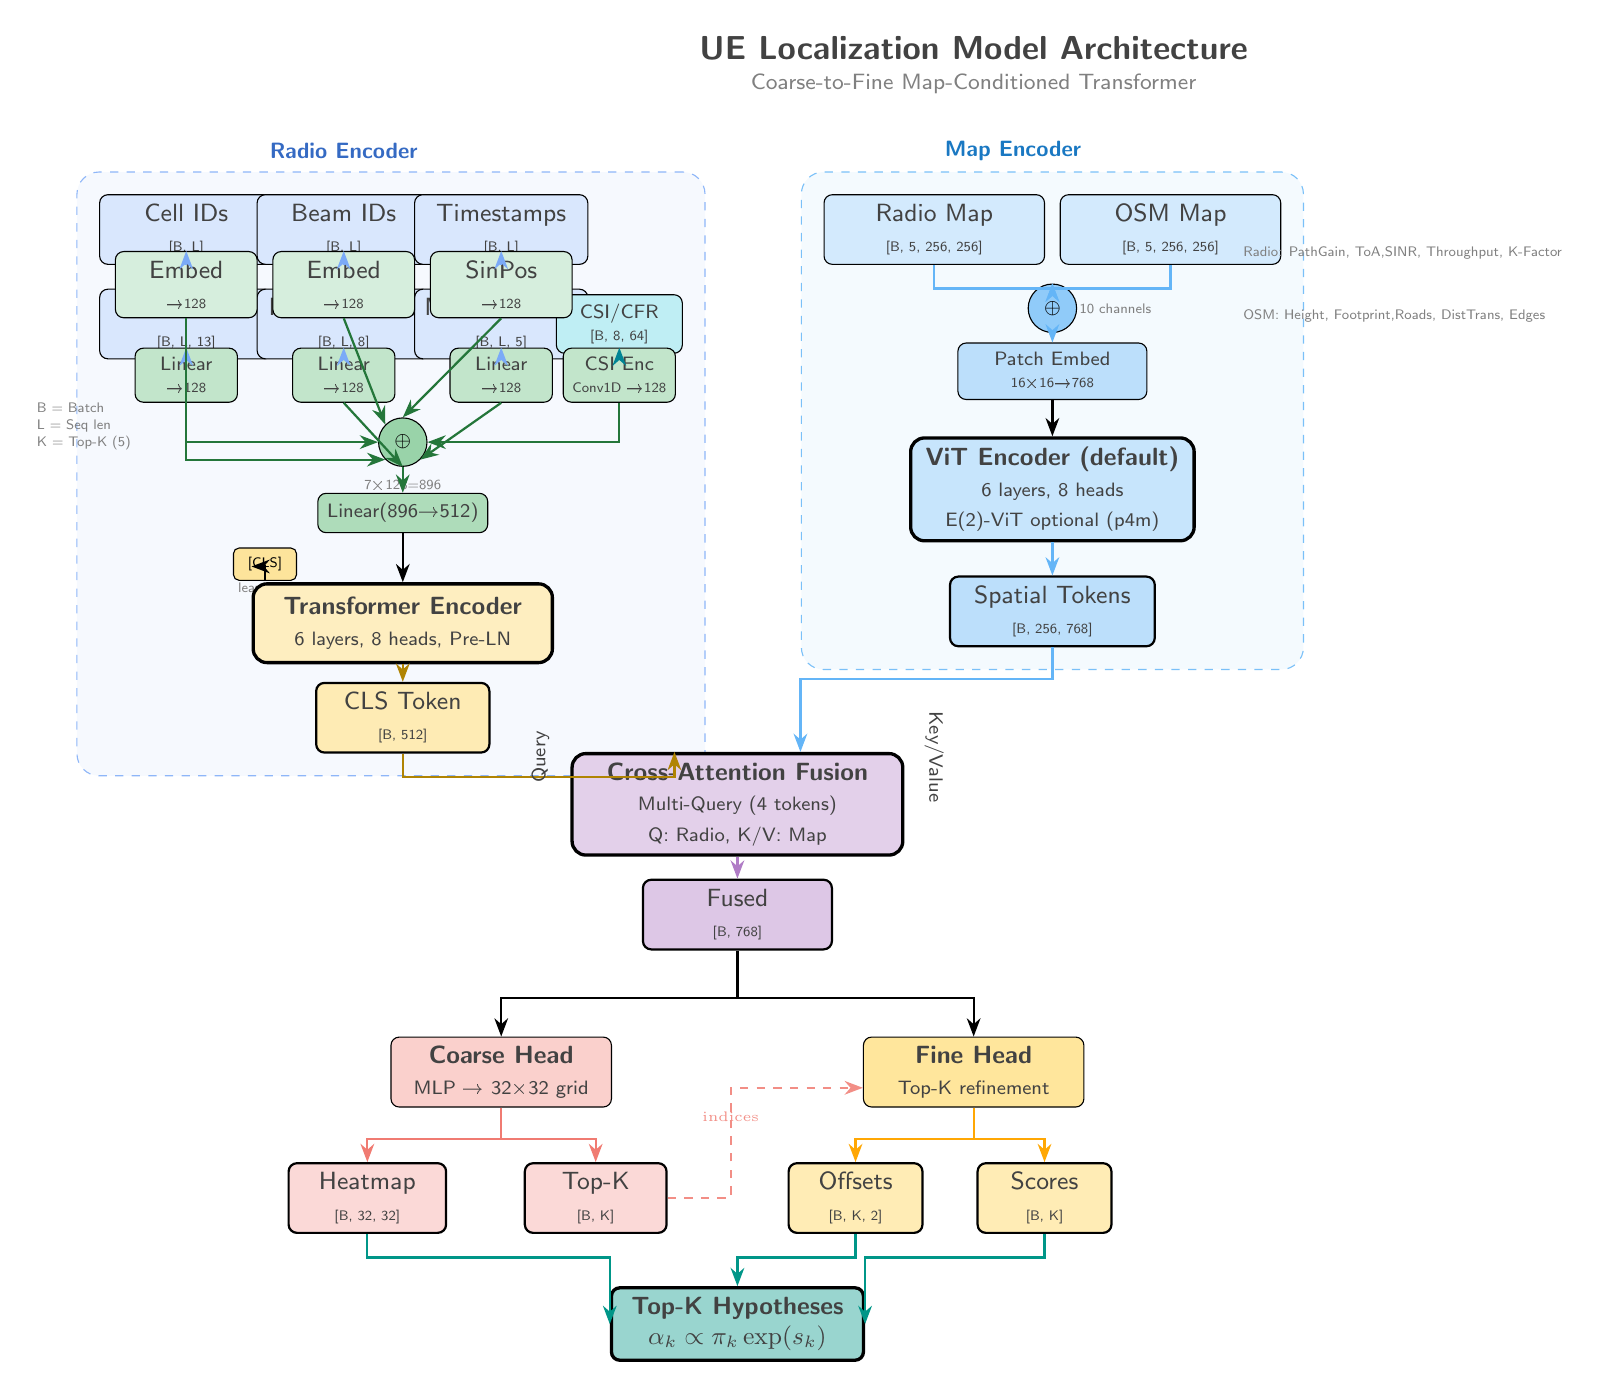
\begin{tikzpicture}[
    node distance=0.6cm and 0.8cm,
    >=Latex,
    font=\sffamily\small,
    % Block styles
    inputbox/.style={draw, rounded corners=3pt, fill=inputblue!20, minimum width=2.2cm, minimum height=0.7cm, align=center, text=darkgray},
    embedbox/.style={draw, rounded corners=3pt, fill=embedgreen!20, minimum width=1.8cm, minimum height=0.6cm, align=center, text=darkgray},
    projbox/.style={draw, rounded corners=3pt, fill=embedgreen!30, minimum width=1.3cm, minimum height=0.5cm, align=center, font=\sffamily\scriptsize, text=darkgray},
    transformer/.style={draw, rounded corners=5pt, fill=transformerorange!25, minimum width=3.2cm, minimum height=1.0cm, align=center, text=darkgray, very thick},
    fusionbox/.style={draw, rounded corners=5pt, fill=fusionpurple!25, minimum width=3.0cm, minimum height=0.9cm, align=center, text=darkgray, very thick},
    headbox/.style={draw, rounded corners=3pt, fill=coarsered!20, minimum width=2.8cm, minimum height=0.8cm, align=center, text=darkgray},
    outputbox/.style={draw, rounded corners=3pt, fill=outputteal!25, minimum width=2.4cm, minimum height=0.7cm, align=center, text=darkgray, thick},
    mapbox/.style={draw, rounded corners=3pt, fill=mapblue!20, minimum width=2.2cm, minimum height=0.7cm, align=center, text=darkgray},
    cfrbox/.style={draw, rounded corners=3pt, fill=cfrcyan!25, minimum width=1.6cm, minimum height=0.5cm, align=center, font=\sffamily\scriptsize, text=darkgray},
    arrow/.style={->, thick, >=Stealth},
    dasharrow/.style={->, thick, >=Stealth, dashed},
    catarrow/.style={->, thick, >=Stealth, color=embedgreen!70!black},
    label/.style={font=\sffamily\scriptsize, text=darkgray},
    dimtext/.style={font=\sffamily\tiny, text=gray},
]

% ============================================
% TITLE
% ============================================
\node[font=\sffamily\bfseries\large, text=darkgray] at (4.5, 8.8) {UE Localization Model Architecture};
\node[font=\sffamily\footnotesize, text=gray] at (4.5, 8.35) {Coarse-to-Fine Map-Conditioned Transformer};

% ============================================
% LEFT SIDE: RADIO ENCODER
% ============================================
\node[font=\sffamily\bfseries\footnotesize, text=inputblue!80!black] at (-3.5, 7.5) {Radio Encoder};

% Input Boxes
\node[inputbox] (cellin) at (-5.5, 6.5) {Cell IDs\\{\tiny [B, L]}};
\node[inputbox] (beamin) at (-3.5, 6.5) {Beam IDs\\{\tiny [B, L]}};
\node[inputbox] (timein) at (-1.5, 6.5) {Timestamps\\{\tiny [B, L]}};

\node[inputbox] (rtin) at (-5.5, 5.3) {RT Features\\{\tiny [B, L, 13]}};
\node[inputbox] (phyin) at (-3.5, 5.3) {PHY Features\\{\tiny [B, L, 8]}};
\node[inputbox] (macin) at (-1.5, 5.3) {MAC Features\\{\tiny [B, L, 5]}};

\node[cfrbox] (cfrin) at (-0.0, 5.3) {CSI/CFR\\{\tiny [B, 8, 64]}};

% Embedding/Projection layers
\node[embedbox] (cellemb) at (-5.5, 5.8) {Embed\\{\tiny →128}};
\node[embedbox] (beamemb) at (-3.5, 5.8) {Embed\\{\tiny →128}};
\node[embedbox] (timeemb) at (-1.5, 5.8) {SinPos\\{\tiny →128}};

\node[projbox] (rtproj) at (-5.5, 4.65) {Linear\\{\tiny →128}};
\node[projbox] (phyproj) at (-3.5, 4.65) {Linear\\{\tiny →128}};
\node[projbox] (macproj) at (-1.5, 4.65) {Linear\\{\tiny →128}};
\node[projbox] (cfrenc) at (0.0, 4.65) {CSI Enc\\{\tiny Conv1D →128}};

% Arrows from inputs to embeddings
\draw[arrow, inputblue!70] (cellin.south) -- (cellemb.north);
\draw[arrow, inputblue!70] (beamin.south) -- (beamemb.north);
\draw[arrow, inputblue!70] (timein.south) -- (timeemb.north);
\draw[arrow, inputblue!70] (rtin.south) -- (rtproj.north);
\draw[arrow, inputblue!70] (phyin.south) -- (phyproj.north);
\draw[arrow, inputblue!70] (macin.south) -- (macproj.north);
\draw[arrow, cfrcyan!70!black] (cfrin.south) -- (cfrenc.north);

% Concatenation node
\node[draw, circle, fill=embedgreen!50, minimum size=0.5cm, font=\sffamily\bfseries\scriptsize] (concat) at (-2.75, 3.8) {$\oplus$};
\node[dimtext, below=0.05cm of concat] {{\tiny 7×128=896}};

% Arrows to concatenation
\draw[catarrow] (cellemb.south) |- (concat.west);
\draw[catarrow] (beamemb.south) -- (concat.north west);
\draw[catarrow] (timeemb.south) -- (concat.north);
\draw[catarrow] (rtproj.south) |- (concat.south west);
\draw[catarrow] (phyproj.south) -- (concat.south);
\draw[catarrow] (macproj.south) -- (concat.south east);
\draw[catarrow] (cfrenc.south) |- (concat.east);

% Linear projection
\node[projbox, minimum width=2.0cm, fill=embedgreen!40] (inputproj) at (-2.75, 2.9) {Linear(896→512)};
\draw[arrow, embedgreen!70!black] (concat.south) -- (inputproj.north);

% CLS Token
\node[draw, rounded corners=2pt, fill=transformerorange!40, minimum width=0.8cm, minimum height=0.4cm, font=\sffamily\tiny] (cls) at (-4.5, 2.25) {[CLS]};
\node[dimtext] at (-4.5, 1.95) {{\tiny learnable}};

% Transformer Encoder
\node[transformer, minimum width=3.8cm] (radioenc) at (-2.75, 1.5) {\textbf{Transformer Encoder}\\{\scriptsize 6 layers, 8 heads, Pre-LN}};
\draw[arrow] (inputproj.south) -- ++(0, -0.25) -| (radioenc.north);
\draw[arrow] (cls.south) |- ([yshift=0.2cm]radioenc.north west);

% CLS output
\node[outputbox, fill=transformerorange!30, minimum width=2.2cm] (radiocls) at (-2.75, 0.3) {CLS Token\\{\tiny [B, 512]}};
\draw[arrow, transformerorange!70!black] (radioenc.south) -- (radiocls.north);

% ============================================
% RIGHT SIDE: MAP ENCODER
% ============================================
\node[font=\sffamily\bfseries\footnotesize, text=mapblue!80!black] at (5.0, 7.5) {Map Encoder};

% Map inputs
\node[mapbox, minimum width=2.8cm] (radiomap) at (4.0, 6.5) {Radio Map\\{\tiny [B, 5, 256, 256]}};
\node[mapbox, minimum width=2.8cm] (osmmap) at (7.0, 6.5) {OSM Map\\{\tiny [B, 5, 256, 256]}};

% Early fusion
\node[draw, circle, fill=mapblue!50, minimum size=0.5cm, font=\sffamily\bfseries\scriptsize] (mapconcat) at (5.5, 5.5) {$\oplus$};
\node[dimtext] at (6.3, 5.5) {{\tiny 10 channels}};
\draw[arrow, mapblue!70] (radiomap.south) -- ++(0, -0.3) -| (mapconcat);
\draw[arrow, mapblue!70] (osmmap.south) -- ++(0, -0.3) -| (mapconcat);

% Patch embedding
\node[projbox, minimum width=2.4cm, fill=mapblue!30] (patchemb) at (5.5, 4.7) {Patch Embed\\{\tiny 16×16→768}};
\draw[arrow, mapblue!70] (mapconcat.south) -- (patchemb.north);

% Map Vision Transformer
\node[transformer, minimum width=3.6cm, fill=mapblue!25] (mapvit) at (5.5, 3.2) {\textbf{ViT Encoder (default)}\\{\scriptsize 6 layers, 8 heads}\\{\scriptsize E(2)-ViT optional (p4m)}};
\draw[arrow] (patchemb.south) -- (mapvit.north);

% Map spatial tokens output
\node[outputbox, fill=mapblue!30, minimum width=2.6cm] (maptokens) at (5.5, 1.65) {Spatial Tokens\\{\tiny [B, 256, 768]}};
\draw[arrow, mapblue!70] (mapvit.south) -- (maptokens.north);

% ============================================
% CENTER: CROSS-ATTENTION FUSION
% ============================================
\node[fusionbox, minimum width=4.2cm, minimum height=1.2cm] (fusion) at (1.5, -0.8) {\textbf{Cross-Attention Fusion}\\{\scriptsize Multi-Query (4 tokens)}\\{\scriptsize Q: Radio, K/V: Map}};

% Arrows to fusion
\draw[arrow, transformerorange!70!black] (radiocls.south) -- ++(0, -0.3) -| ([xshift=-0.8cm]fusion.north);
\draw[arrow, mapblue!70] (maptokens.south) -- ++(0, -0.4) -| ([xshift=0.8cm]fusion.north);

% Labels
\node[label, rotate=90] at (-1.0, -0.2) {Query};
\node[label, rotate=-90] at (4.0, -0.2) {Key/Value};

% Fused output
\node[outputbox, fill=fusionpurple!30, minimum width=2.4cm] (fused) at (1.5, -2.2) {Fused\\{\tiny [B, 768]}};
\draw[arrow, fusionpurple!70] (fusion.south) -- (fused.north);

% ============================================
% BOTTOM: PREDICTION HEADS
% ============================================
% Coarse Head
\node[headbox, fill=coarsered!25] (coarse) at (-1.5, -4.2) {\textbf{Coarse Head}\\{\scriptsize MLP → 32×32 grid}};
\draw[arrow] (fused.south) -- ++(0, -0.6) -| (coarse.north);

% Fine Head
\node[headbox, fill=fineyellow!40] (fine) at (4.5, -4.2) {\textbf{Fine Head}\\{\scriptsize Top-K refinement}};
\draw[arrow] (fused.south) -- ++(0, -0.6) -| (fine.north);

% Coarse outputs
\node[outputbox, fill=coarsered!20, minimum width=2.0cm] (heatmap) at (-3.2, -5.8) {Heatmap\\{\tiny [B, 32, 32]}};
\node[outputbox, fill=coarsered!20, minimum width=1.8cm] (topk) at (-0.3, -5.8) {Top-K\\{\tiny [B, K]}};
\draw[arrow, coarsered!70] (coarse.south) -- ++(0, -0.4) -| (heatmap.north);
\draw[arrow, coarsered!70] (coarse.south) -- ++(0, -0.4) -| (topk.north);

% Connection from coarse to fine (top-k indices)
\draw[dasharrow, coarsered!60] (topk.east) -- ++(0.8, 0) |- ([yshift=-0.2cm]fine.west) node[pos=0.3, above, font=\tiny] {indices};

% Fine outputs
\node[outputbox, fill=fineyellow!30, minimum width=1.7cm] (offsets) at (3.0, -5.8) {Offsets\\{\tiny [B, K, 2]}};
\node[outputbox, fill=fineyellow!30, minimum width=1.7cm] (scores) at (5.4, -5.8) {Scores\\{\tiny [B, K]}};
\draw[arrow, fineyellow!60!orange] (fine.south) -- ++(0, -0.4) -| (offsets.north);
\draw[arrow, fineyellow!60!orange] (fine.south) -- ++(0, -0.4) -| (scores.north);

% ============================================
% FINAL OUTPUT
% ============================================
\node[outputbox, fill=outputteal!40, minimum width=3.2cm, minimum height=0.8cm, very thick] (finalpos) at (1.5, -7.4) {\textbf{Top-K Hypotheses}\\$\alpha_k \propto \pi_k \exp(s_k)$};
\draw[arrow, thick, outputteal] (heatmap.south) |- ++(0, -0.3) -| (finalpos.west);
\draw[arrow, thick, outputteal] (offsets.south) |- ++(0, -0.3) -| (finalpos);
\draw[arrow, thick, outputteal] (scores.south) |- ++(0, -0.3) -| (finalpos.east);

% ============================================
% ANNOTATIONS/LEGEND
% ============================================
% Dashed box around radio encoder
\begin{scope}[on background layer]
    \node[draw=inputblue!60, dashed, rounded corners=8pt, fit=(cellin)(cfrin)(radioenc)(radiocls), inner sep=8pt, fill=inputblue!5] {};
\end{scope}

% Dashed box around map encoder  
\begin{scope}[on background layer]
    \node[draw=mapblue!60, dashed, rounded corners=8pt, fit=(radiomap)(osmmap)(mapvit)(maptokens), inner sep=8pt, fill=mapblue!5] {};
\end{scope}

% Dimension annotations
\node[font=\sffamily\tiny, text=gray, align=left] at (-6.8, 4.0) {B = Batch\\L = Seq len\\K = Top-K (5)};

% Channel annotations for maps
\node[font=\sffamily\tiny, text=gray, right] at (7.8, 6.2) {Radio: PathGain, ToA,\\SINR, Throughput, K-Factor};
\node[font=\sffamily\tiny, text=gray, right] at (7.8, 5.4) {OSM: Height, Footprint,\\Roads, DistTrans, Edges};

\end{tikzpicture}
\end{document}
